\documentclass[11pt,a4paper]{article}
\usepackage[utf8x]{inputenc}
\usepackage{ucs}
\usepackage{amsmath}
\usepackage{amsfonts}
\usepackage{amssymb}
\usepackage{url}
\usepackage{graphicx}
\usepackage{subfigure}


\author{HU, Pili \\
MobiTeC, IE Department, CUHK \\
\texttt{hupili@ie.cuhk.edu.hk} \\
\url{http://personal.ie.cuhk.edu.hk/~hpl011/} 
}

\title{Adaptive Video Streaming: 
 \\ a Survey and Case Study}

\begin{document}

\maketitle

\begin{abstract}
	In the past decade, Internet traffic has seen a significant 
	change from web browsing to video viewing. The ongoing trend 
	raises a chanllenging problem: how to stream data to heterogeous 
	peers? 
	
	The designer of such data streaming architecture should 
	bear the following considerations in mind: QoE, server load, 
	network resource efficiency, scalability, etc. The heterogeneous 
	peer network condition makes the design more complicated. The 
	underlying codec ranges from Multi Description Coding to Multi 
	Layer Coding. The data deliver architecture ranges from unicast,
	multicast, to P2P network. Researchers have focused on different 
	system settings and optimization objectives. 
	 
	This paper will first
	sum up several works in the context of adaptive video streaming. 
	At the same time, we do a case study on a commercial adaptive 
	video streaming system, which combines Multilayer Codec and P2P 
	technology. Possible improvements on this system are proposed
	with reasoning. Some of the conjectures are
	verified through a corresponding simulation platform based on NS2. 
\end{abstract}

\pagebreak
\tableofcontents
\pagebreak

\section{Introduction}



\begin{itemize}
	\item User perceived experience. 
	\item Vendor cost. 
	\item User cost. 
	\item System cost. 
\end{itemize}

\section{General Model}


\section{Problem Scope}

\subsection{Codec}

\subsection{Networking}

\section{Design of Adaptive P2P VoD System}


\subsection{Codec Choice}

\subsection{Transimission Protocol Choice}


\subsection{Overlay Construction}

\subsection{Peer Selection}


\subsection{Buffer Management}


\subsection{Chunck Selection}

MMKP, Knapsack

MCMF, Network Flow 



\subsection{Playback Decision}


\subsection{User Model}



\section{A Case Study and Simulation }

\subsection{Baseline Description}

\begin{figure}[htb]
	\centering
	\includegraphics[width=0.6\textwidth]{../fig/version_tree.png}
	\caption{Version Tree of Real and Simulation}
\end{figure}

\begin{itemize}
	\item Blue: Real deployment
	\item While: Simulation platform 
	\item Green: This work  
	\item Red dash: Equivalency
\end{itemize}

\begin{figure}
	\includegraphics[width=0.8\textwidth]{../fig/runtime_vs_core.jpg}
\end{figure}

\begin{figure}
	\includegraphics[width=0.8\textwidth]{../fig/runtime_vs_nodenum.jpg}
\end{figure}

\begin{figure}
	\includegraphics[width=0.8\textwidth]{../fig/runtime_vs_simutime.jpg}
\end{figure}

\begin{itemize}
	\item Number of Nodes: 160
	\item Simulation Time: 300 (NS seconds)
\end{itemize}

Wen Zheng's configuration:
\begin{itemize}
	\item Star like, 4 subnet. 
	\item Subnet parameters:
		\begin{itemize}
			\item Subnet1: down:10Mb; up:10Mb. 
			\item Subnet1: down:3Mb; up:0.5Mb. 
			\item Subnet1: down:3Mb; up:0.5Mb. 
			\item Subnet1: down:3Mb; up:0.5Mb. 
		\end{itemize}
\end{itemize}

\begin{itemize}
	\item 3 Layers. Conform to [wang,2011] QoE study.  
	\item Layer parameters:
		\begin{itemize}
			\item Layer1: 256Kbit. (per piece) 
			\item Layer2: 256Kbit. (per piece) 
			\item Layer3: 512Kbit. (per piece) 
		\end{itemize}
\end{itemize}

\subsection{QoE Model Implementation}

[wang, 2011], B-D tradeoff, continuous version. 
\begin{equation}
	MOS = c_1 \times d + \alpha \times (1 - e^{-b \times \lambda}) + c_2
\end{equation}
\begin{figure}
	\subfigure[3D]{
	\includegraphics[width=0.45\textwidth]{../fig/bd_3d.jpg}
	}
	\subfigure[contour]{
	\includegraphics[width=0.45\textwidth]{../fig/bd_contour.jpg}
	}
	\caption{Conclusion, QoE and Performance}
\end{figure}


\subsection{Baseline Test}

\begin{figure}
	\includegraphics[width=0.8\textwidth]{../fig/simutime_qoe.jpg}
\end{figure}

\begin{figure}
	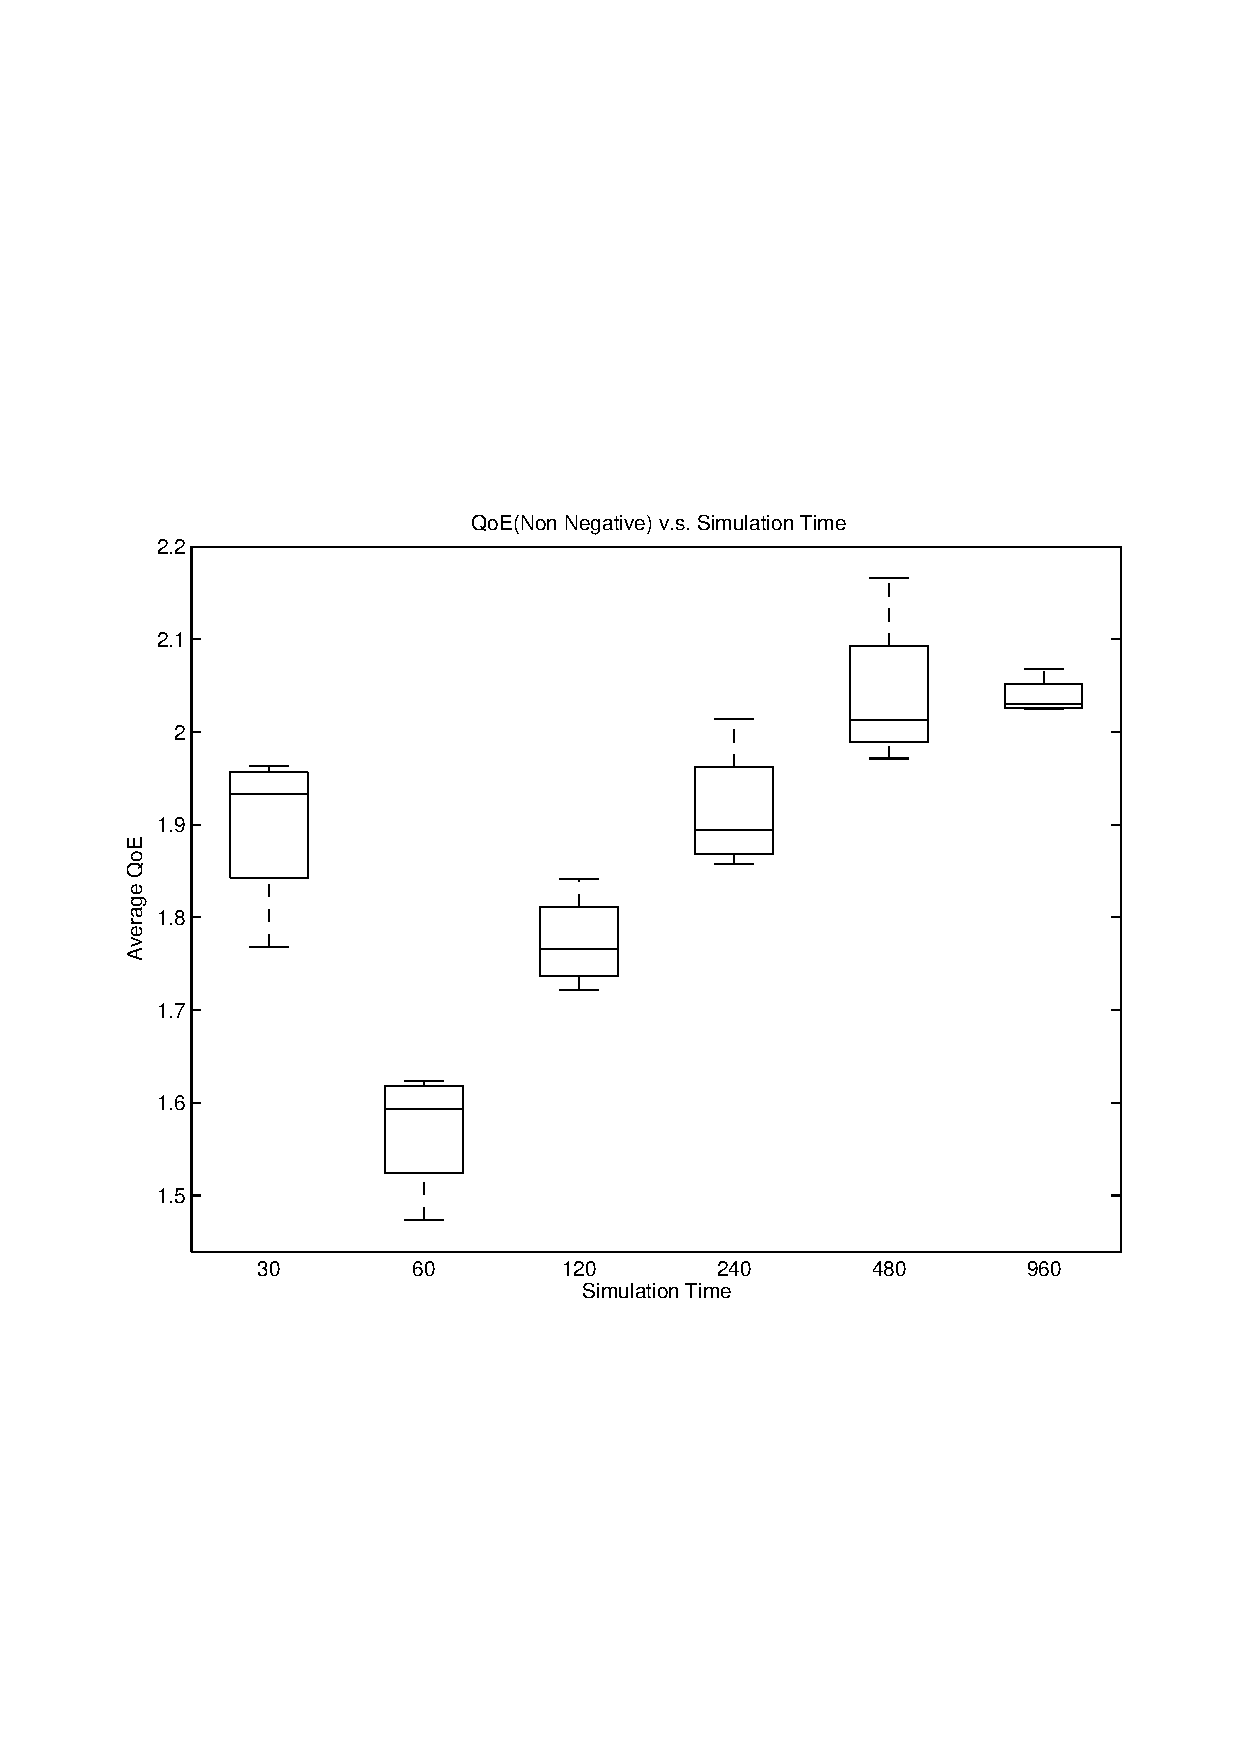
\includegraphics[width=0.8\textwidth]{../fig/simutime_qoe_nonneg.jpg}
\end{figure}


\begin{itemize}
      \item     $'count\_mr' => 3749$
      \item     $'count\_mr\_nonneg' => 2601$
      \item     $'avg\_qoe' => '0.871540677419684'$
      \item     $'avg\_qoe\_nonneg' => '2.01996612593628'$
      \item     $'node\_num' => '160'$
      \item     $'simu\_time' => '480'$
      \item     $'core\_num' => '4'$
      \item     $'task\_duration' => 8399$
      \item     $'pdns\_duration' => 8302$
\end{itemize}

\begin{figure}
	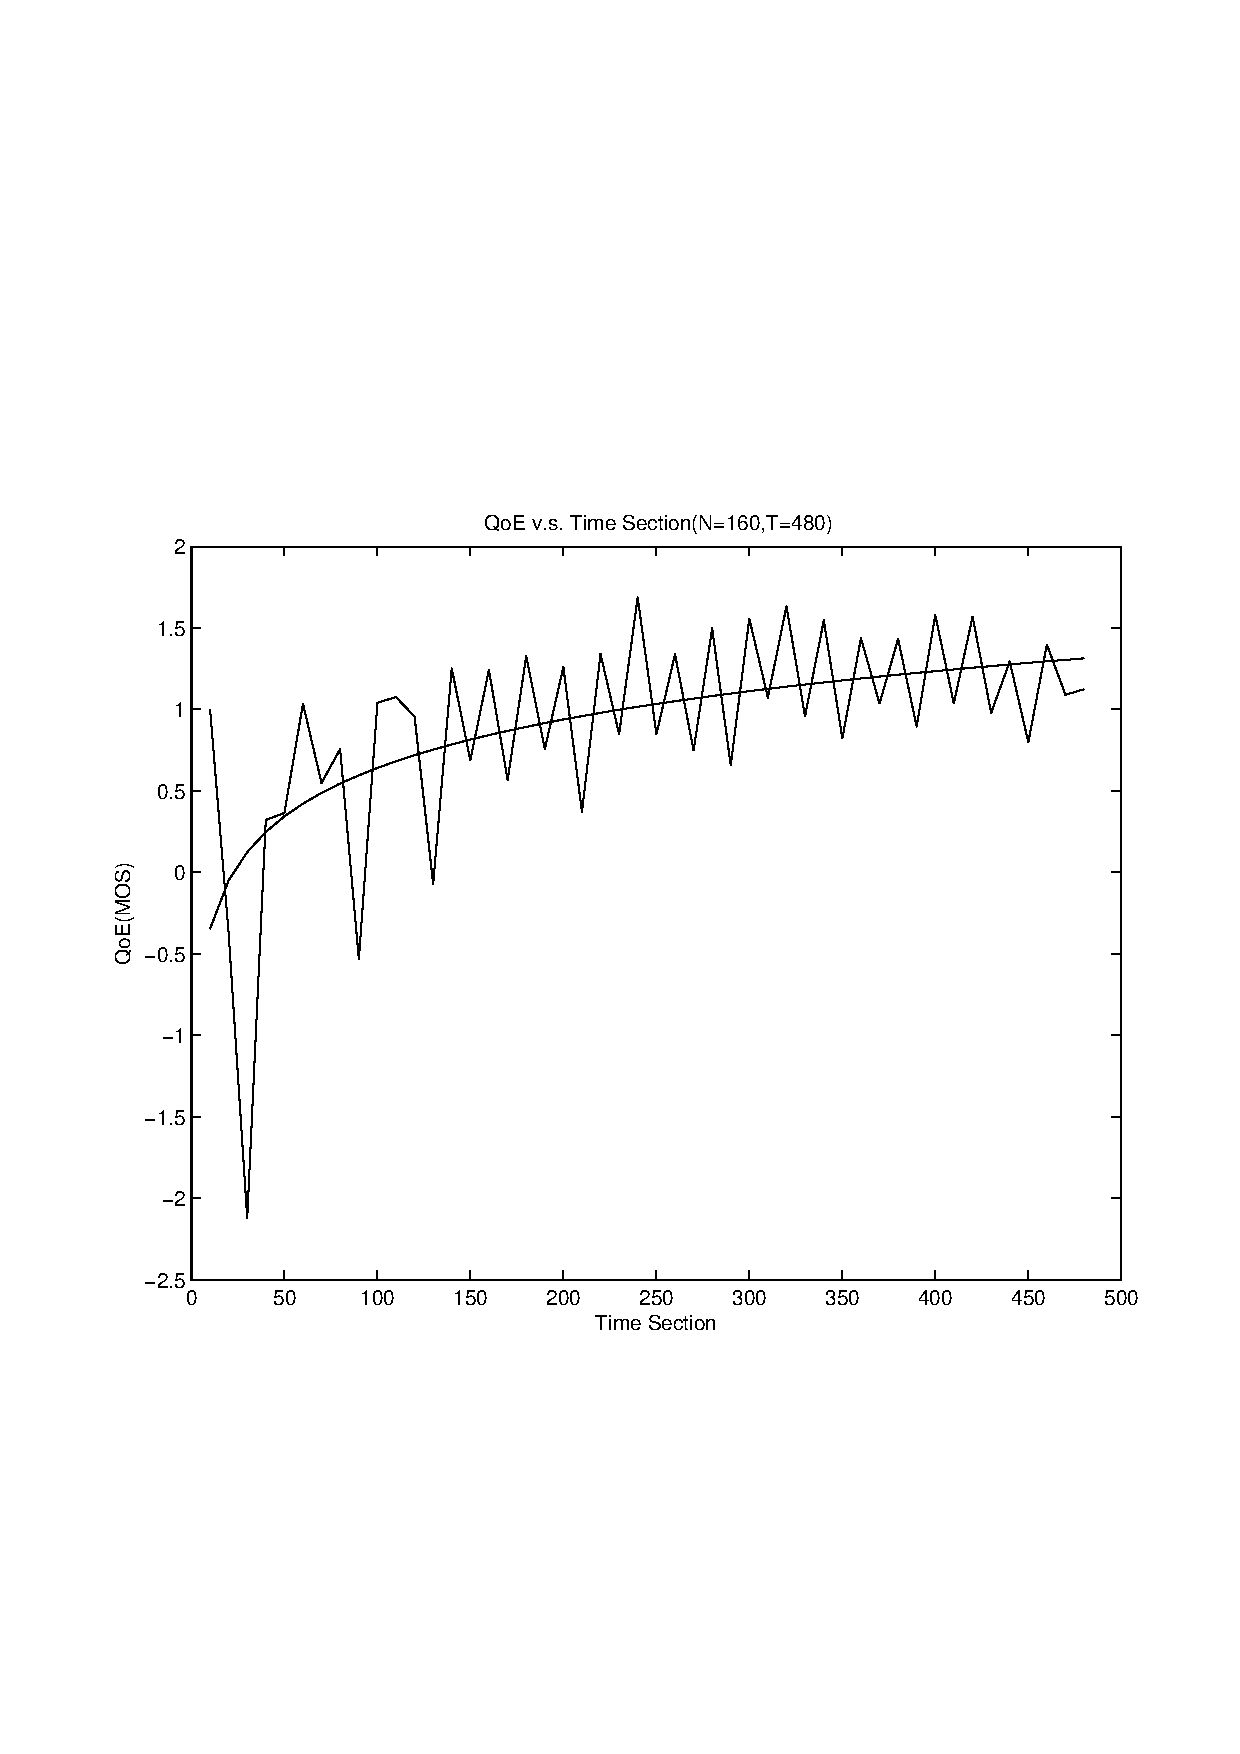
\includegraphics[width=0.6\textwidth]{../fig/time_qoe.jpg}
\end{figure}
Observations:
\begin{itemize}
	\item System bootstraping stage. 
	\item Steady after about 250 seconds. 
\end{itemize}

\begin{figure}
	\includegraphics[width=0.7\textwidth]{../fig/qoe_hist.jpg}
\end{figure}

\subsection{Chunk Selection Architecture Reconstruction}

\begin{figure}
	\includegraphics[width=0.7\textwidth]{../fig/arch_orig.png}
	\caption{Original Architecture}
\end{figure}

\begin{figure}
	\includegraphics[width=0.7\textwidth]{../fig/arch_improved.png}
	\caption{Improved Architecture}
\end{figure}


\begin{figure}
	\includegraphics[width=0.7\textwidth]{../fig/pals_like.png}
	\caption{Improved Architecture}
\end{figure}
Effect:
\begin{itemize}
	\item QoE: 0.7 $\rightarrow$ 3.3
\end{itemize}


\subsection{Priority Based Upgrade}

\begin{table}
\caption{A Sample Priority Table with Window Size = 5}
	\begin{tabular}{|c|ccccc|}
	\hline
	 & t1 & t2 & t3 & t4 & t5 \\
	 \hline
	layer3 & 11 & 12 & 13 & 14 & 15 \\
	layer2 & 6 & 7 & 8 & 9 & 10 \\
	layer1 & 1 & 2 & 3 & 4 & 5 \\
	\hline
	\end{tabular}
\end{table}

Result:
\begin{itemize}
	\item QoE: nearly the same. 
	\item Performance: decrease slightly. 
\end{itemize}



\subsection{Scalable Window Size}

Reason:
\begin{itemize}
	\item From trace, many powerful peeers can get full 3 layers
	in the whole window. 
	\item Give them a chance to download more, and their data
	far from playback pointer can server others. 
\end{itemize}
\begin{table}
\caption{A Sample Priority Table with Window Size = 5+5}
	\begin{tabular}{|c|ccccc|c|}
	\hline
	 & t1 & t2 & t3 & t4 & t5 & t6-t10 \\
	 \hline
	layer3 & 11 & 12 & 13 & 14 & 15 & ...\\
	layer2 & 6 & 7 & 8 & 9 & 10 & ... \\
	layer1 & 1 & 2 & 3 & 4 & 5  & ...\\
	\hline
	\end{tabular}
\end{table}

\begin{table}
\caption{A Sample Priority Table with Window Size = 5+5}
	\begin{tabular}{|c|ccccc|c|}
	\hline
	 & t1 & t2 & t3 & t4 & t5 & t6-t10 \\
	 \hline
	layer3 & 11 & 12 & 13 & 14 & 15 & ...\\
	layer2 & 6 & 7 & 8 & 9 & 10 & ... \\
	layer1 & 1 & 2 & 3 & 4 & 5  & ...\\
	\hline
	\end{tabular}
\end{table}

\subsection{Performance Optimization}

\begin{figure}
	\subfigure{
	\includegraphics[width=0.6\textwidth]{../fig/gprof1.png}
	} \\
	\subfigure{
	\includegraphics[width=0.6\textwidth]{../fig/gprof2.png}
	}
	\caption{GNU Profile, Output}
\end{figure}

Result:
\begin{itemize}
	\item QoE: nearly the same. 
	\item Performance: 4.5h $\rightarrow$ 3.5h. 
\end{itemize}

\subsection{Introduce Randomness in Second Window Section}

Result:
\begin{itemize}
	\item QoE: worse. 
	\item Performance: worse. 
\end{itemize}

\subsection{Conclusion of the Case Study}

\begin{figure}
	\subfigure[qoe]{
	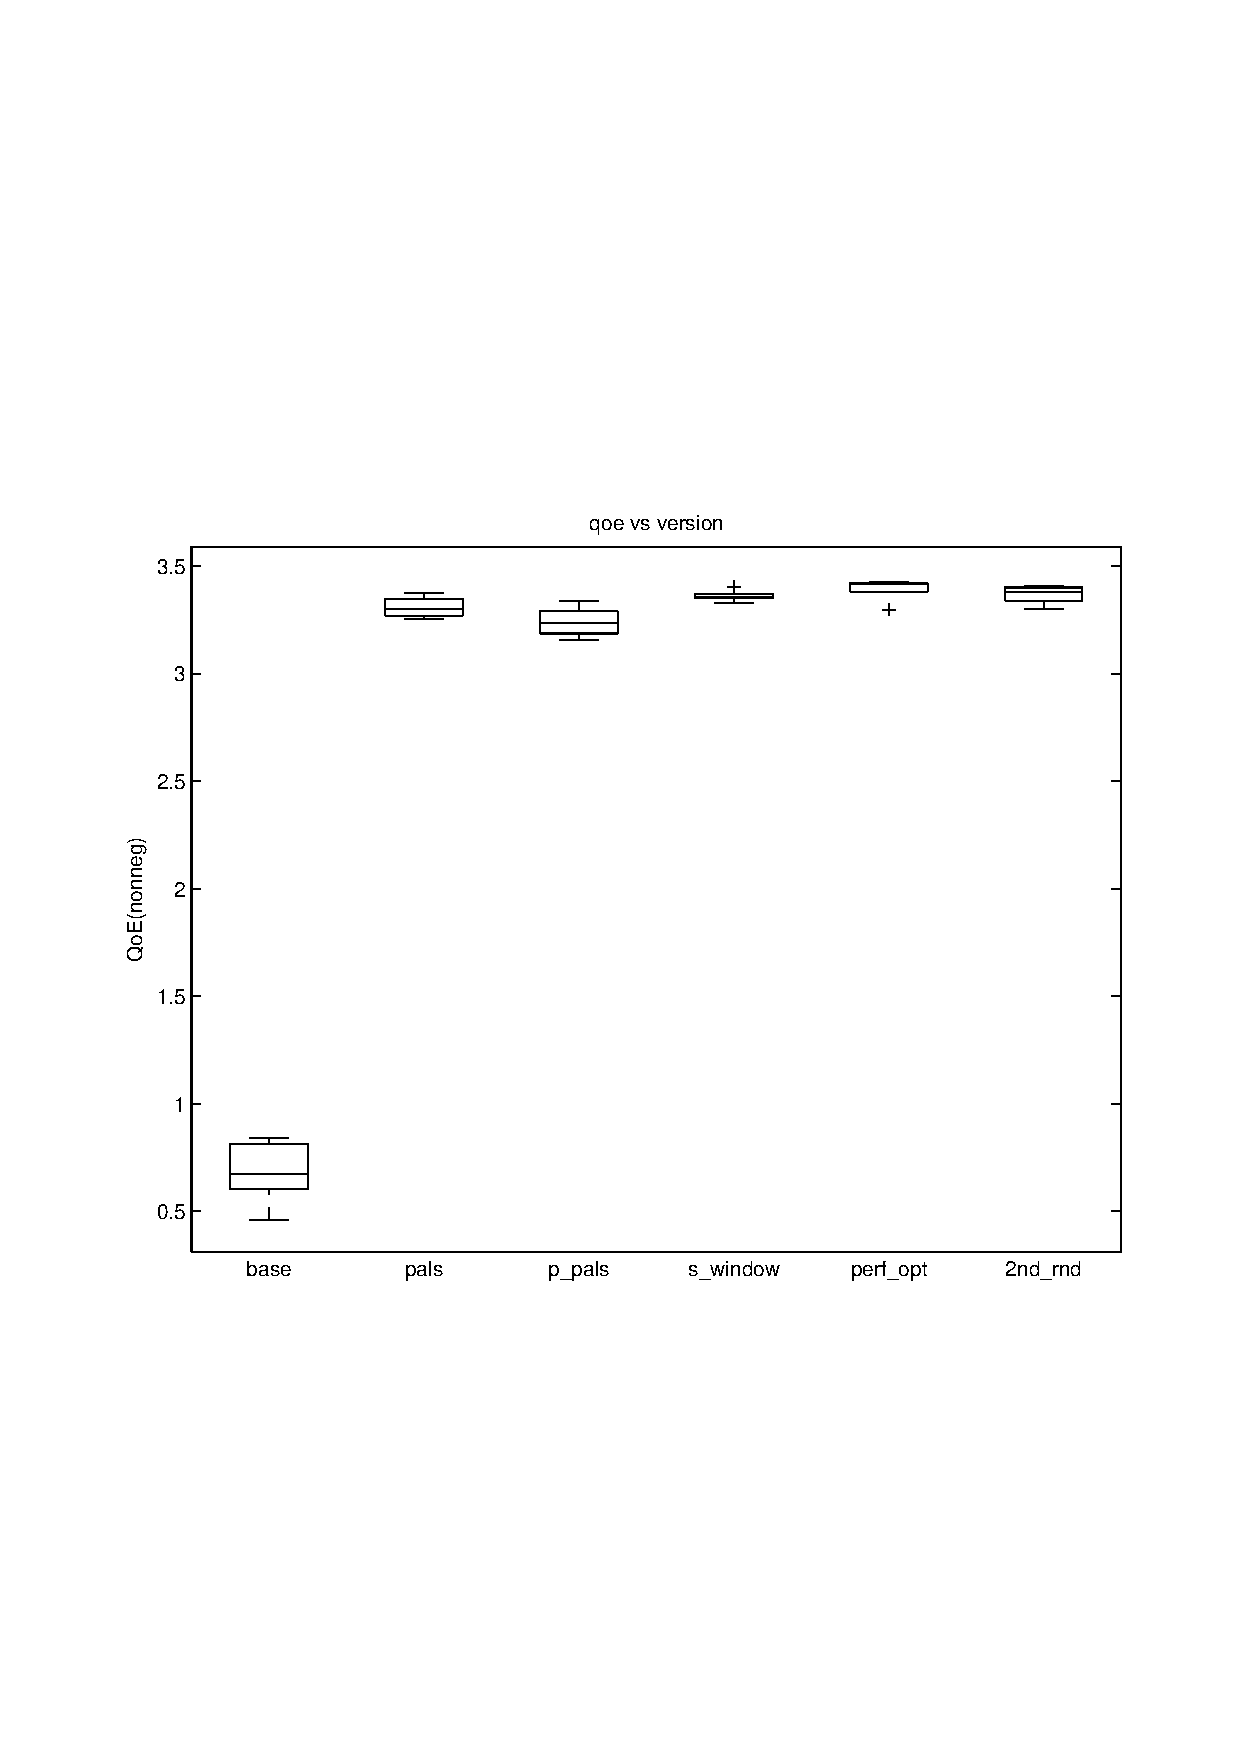
\includegraphics[width=0.45\textwidth]{../fig/con_qoe_version_all.jpg}
	}
	\subfigure[time]{
	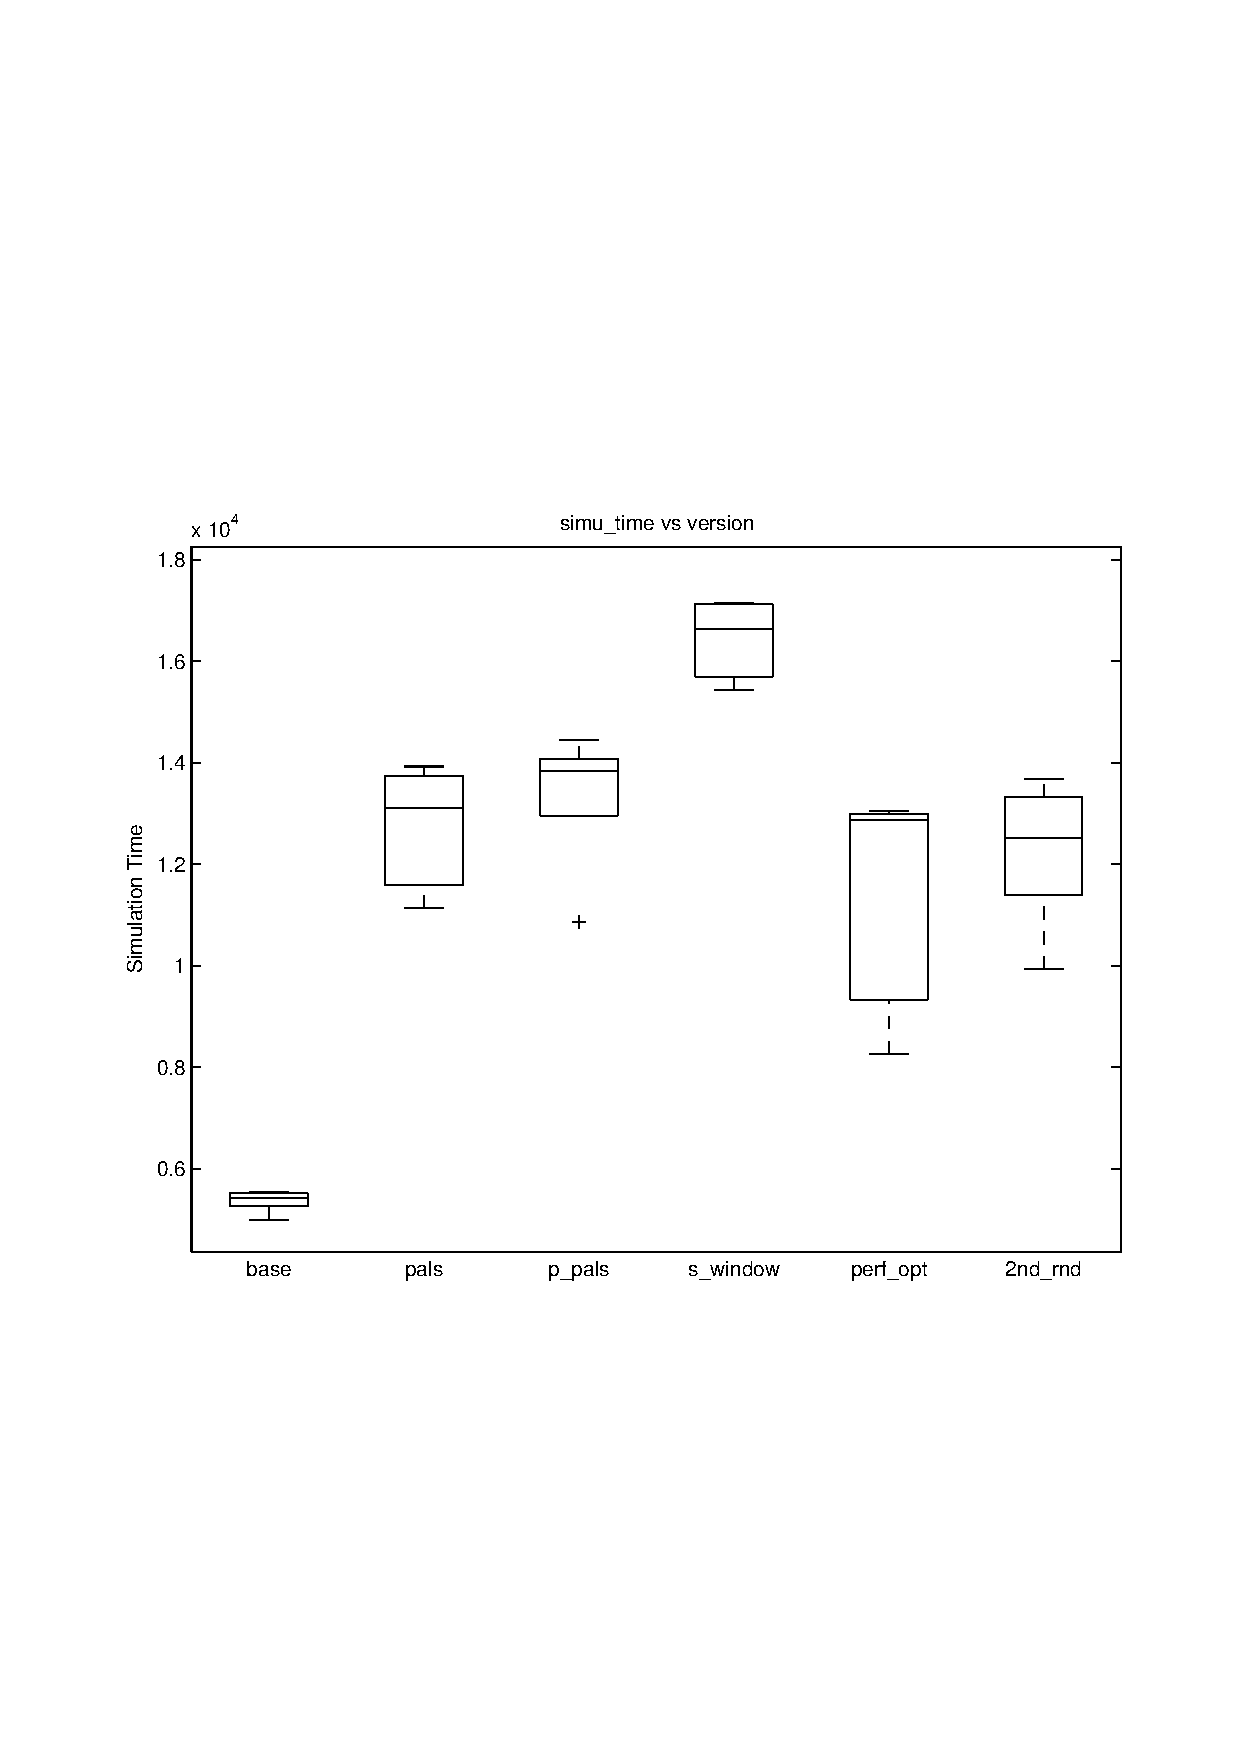
\includegraphics[width=0.45\textwidth]{../fig/con_time_version_all.jpg}
	}
	\caption{Conclusion, QoE and Performance}
\end{figure}

\begin{figure}
	\subfigure[qoe]{
	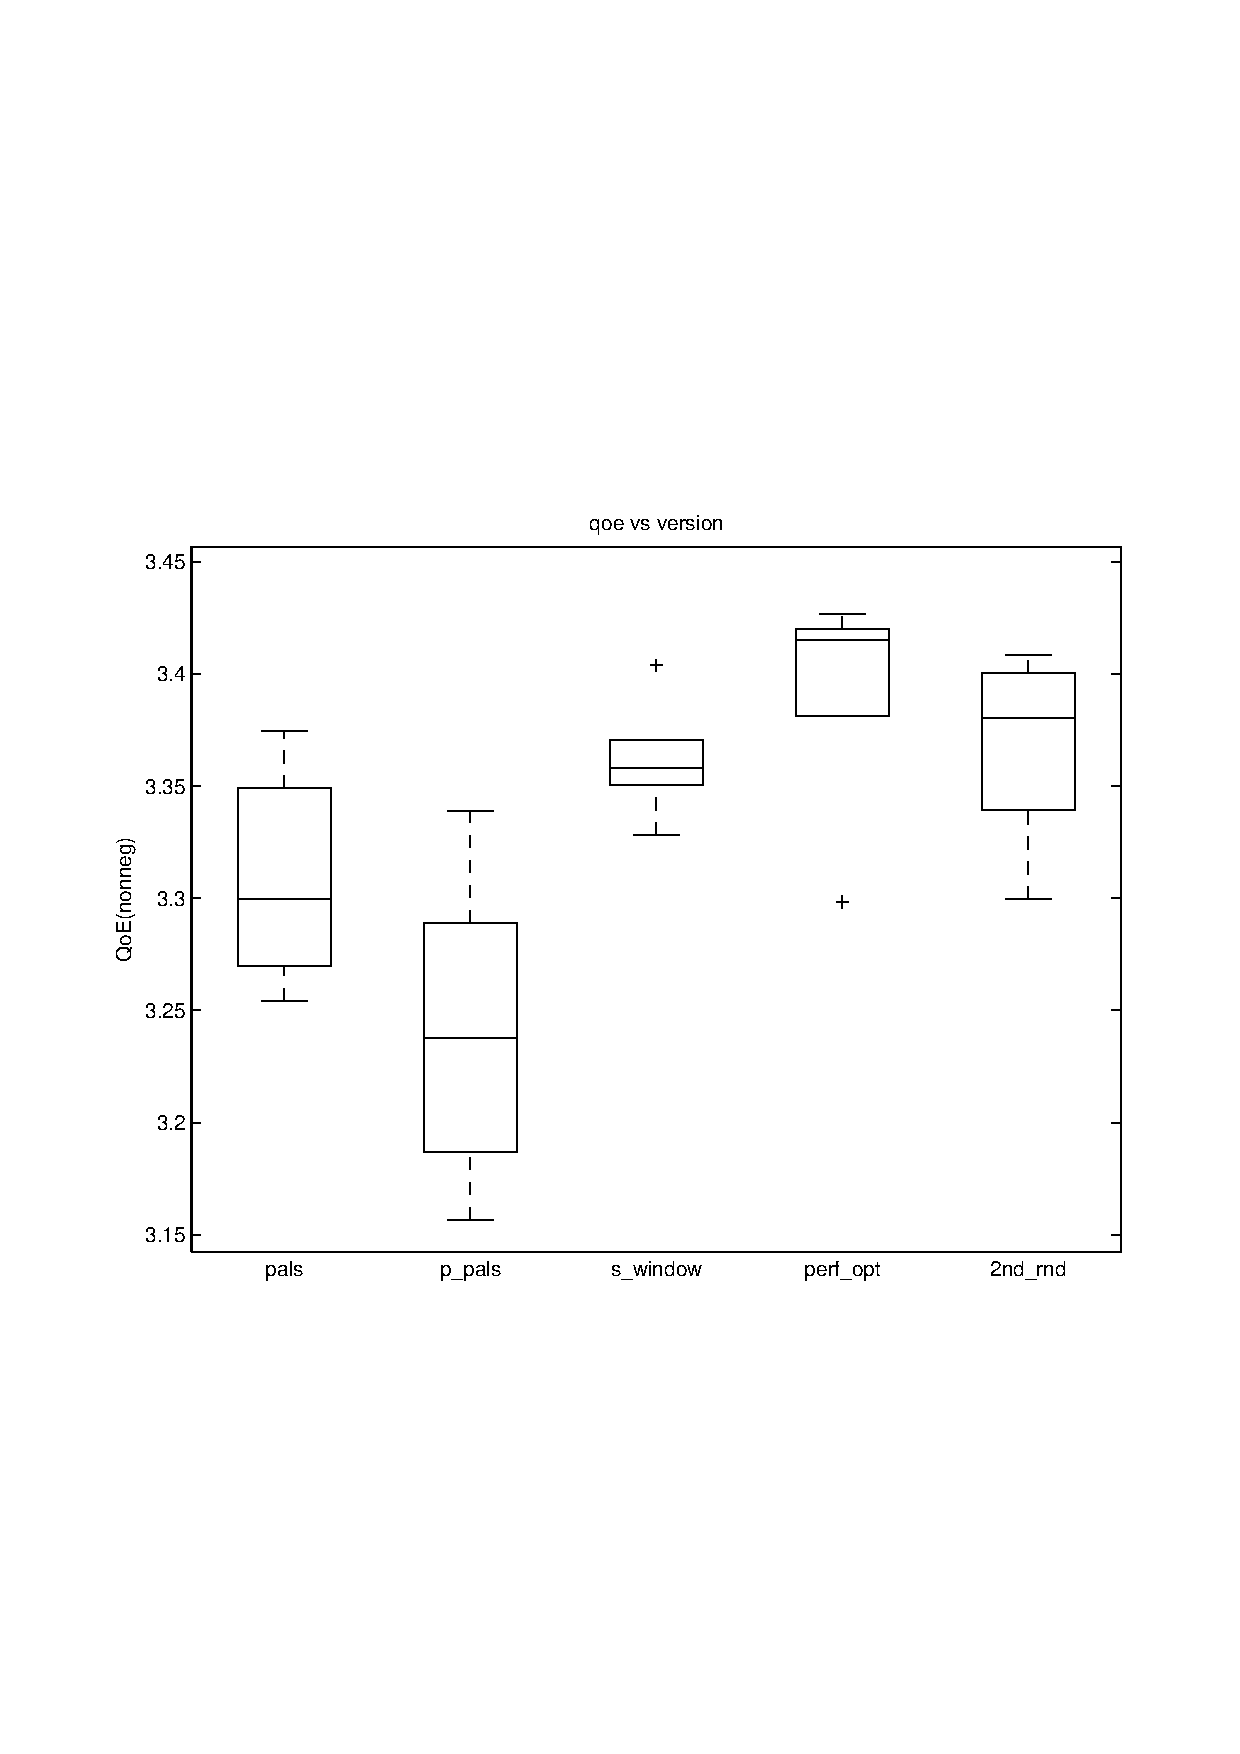
\includegraphics[width=0.45\textwidth]{../fig/con_qoe_version_part.jpg}
	}
	\subfigure[time]{
	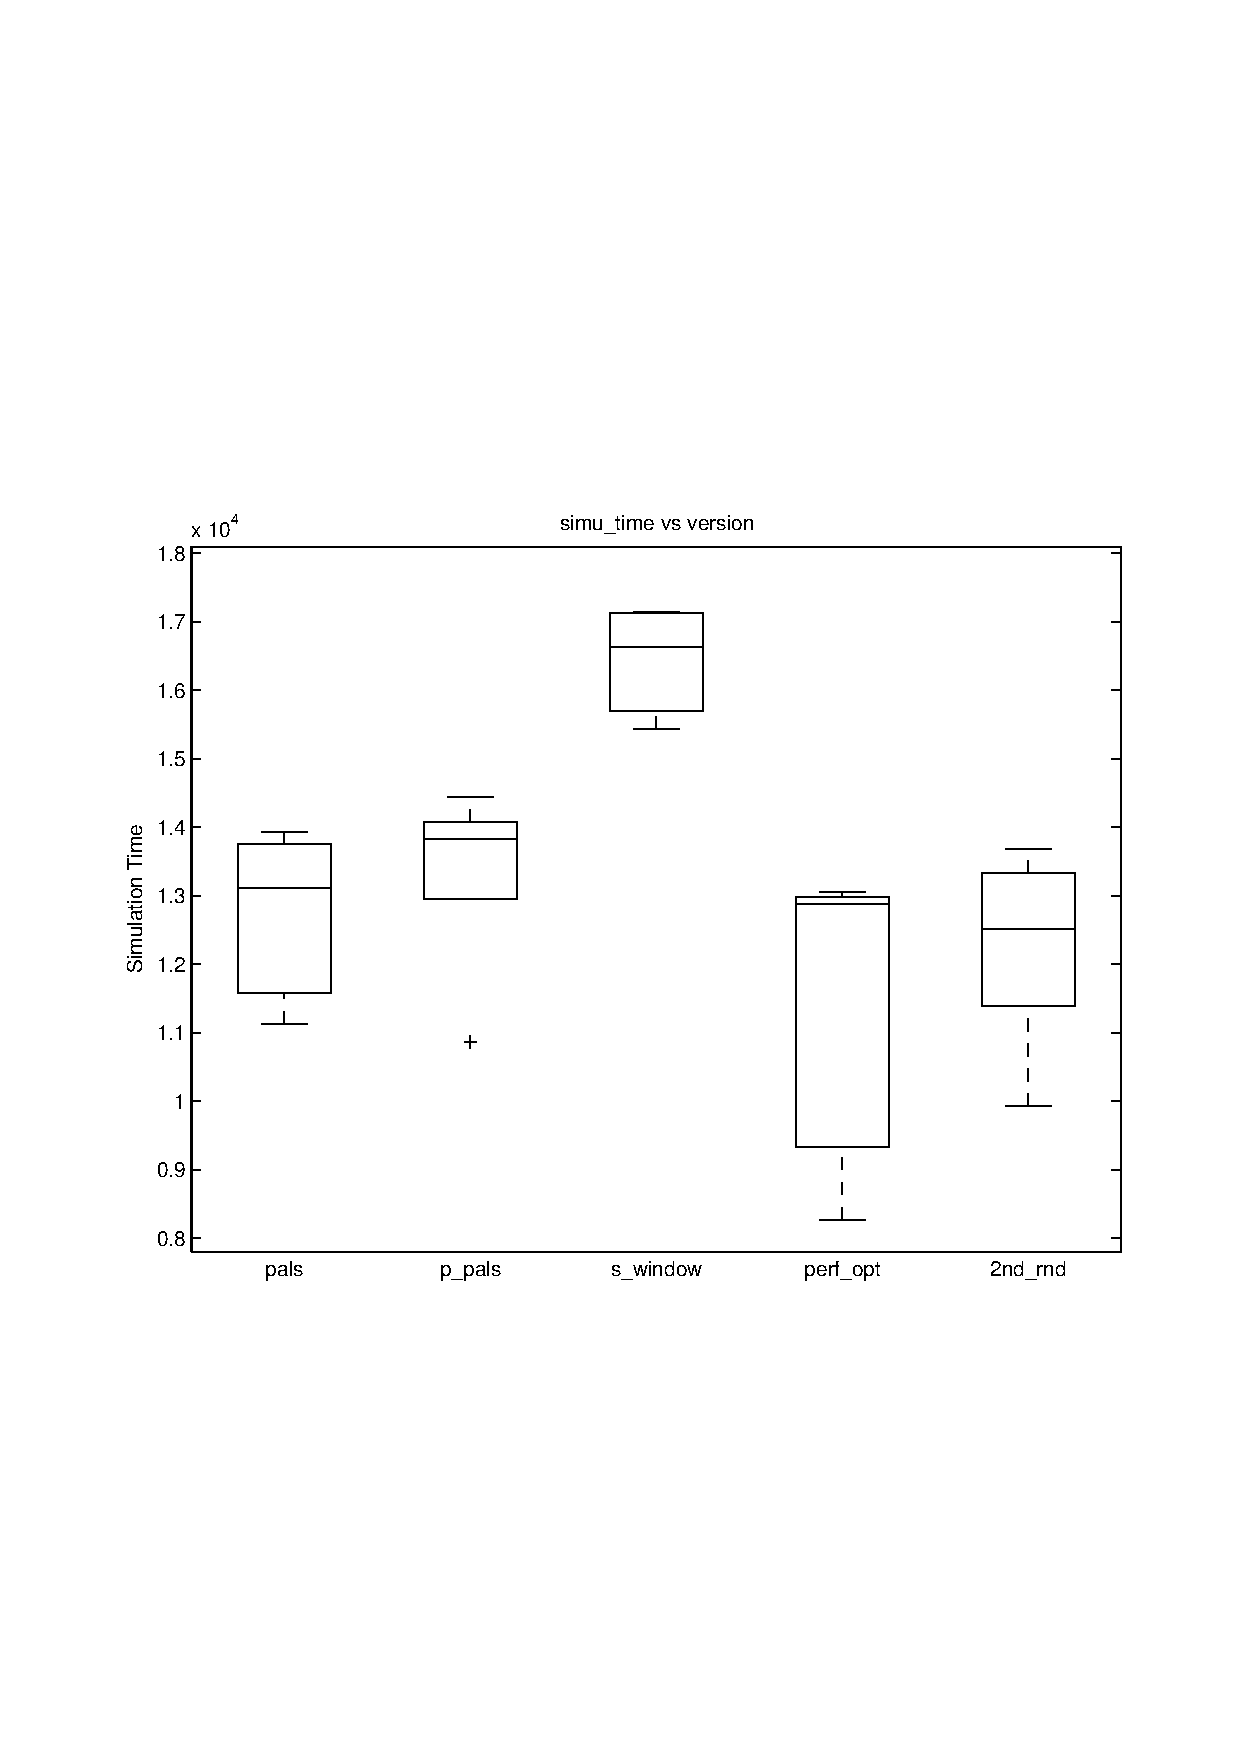
\includegraphics[width=0.45\textwidth]{../fig/con_time_version_part.jpg}
	}
	\caption{Conclusion, QoE and Performance}
\end{figure}



\section{Conclusion}

	\begin{itemize}
		\item Engineering approach v.s. academic approach:\\
		where is the biggest cake? 
		\item Time distribution:
			\begin{itemize}
				\item 70\%, literature survey.(30+ papers) 
				\item 15\%, bugfix of the platform, environment setup. 
				\item 5\%, first unified version(QoE:0.7$\rightarrow$3.3, 
				biggest improvement in this study)
				\item 10\%, scalable window, performance optimization, random 
				2nd section. (little outcome)
			\end{itemize}
	\end{itemize}

\begin{itemize}
	\item 6 big versions / 240 runs. 
	\item Auxilary Scripts:
	\begin{itemize}
	\item .sh:298 lines
	\item .pl:791  lines
	\item .m:133 lines
	\end{itemize}
	\item Simulation Code Difference:	
	\begin{itemize}
		\item download\_agent.cc: 1940 lines
		\item download\_agent.h: 301 lines
		\item labtesting.tcl: 84 lines
	\end{itemize}
\end{itemize}


\section{Future Works}





\section*{Acknowledgements}
\addcontentsline{toc}{section}{Acknowledgements}




\pagebreak
\section*{Appendix}
\addcontentsline{toc}{section}{Appendix}


\pagebreak
\addcontentsline{toc}{section}{References}
\input{gen_bib.bbl}


\end{document}